\documentclass{article}

\usepackage{bm}
\usepackage{graphicx}
\usepackage{amsmath}
\usepackage{amsfonts}
\usepackage{amssymb}
% if you need to pass options to natbib, use, e.g.:
\PassOptionsToPackage{numbers, compress}{natbib}
% before loading neurips_2019

% ready for submission
% \usepackage{neurips_2019}

% to compile a preprint version, e.g., for submission to arXiv, add add the
% [preprint] option:
     \usepackage[preprint]{neurips_2019}

% to compile a camera-ready version, add the [final] option, e.g.:
%     \usepackage[final]{neurips_2019}

% to avoid loading the natbib package, add option nonatbib:
%     \usepackage[nonatbib]{neurips_2019}

\usepackage[utf8]{inputenc} % allow utf-8 input
\usepackage[T1]{fontenc}    % use 8-bit T1 fonts
\usepackage{hyperref}       % hyperlinks
\usepackage{url}            % simple URL typesetting
\usepackage{booktabs}       % professional-quality tables
\usepackage{amsfonts}       % blackboard math symbols
\usepackage{nicefrac}       % compact symbols for 1/2, etc.
\usepackage{microtype}      % microtypography

\title{A Hierarchical Inhomogeneous Hidden Markov Model for Cancer Screening Modeling}

% The \author macro works with any number of authors. There are two commands
% used to separate the names and addresses of multiple authors: \And and \AND.
%
% Using \And between authors leaves it to LaTeX to determine where to break the
% lines. Using \AND forces a line break at that point. So, if LaTeX puts 3 of 4
% authors names on the first line, and the last on the second line, try using
% \AND instead of \And before the third author name.

\author{%
  Rui Meng\thanks{Use footnote for providing further information
    about author (webpage, alternative address)---\emph{not} for acknowledging
    funding agencies.} \\
  Department of Statistics\\
  University of California\\
  Santa Cruz, CA 95060 \\
  \texttt{rmeng1@ucsc.edu} \\
  % examples of more authors
   \And
   Braden Soper \\
   Lawrence Livermore National Laboratory \\
   Livermore, CA \\
   \texttt{soper3@llnl.gov} \\
   \AND
   Jan F. Nygard \\
   Cancer Registry of Norway \\
   Oslo, Norway \\
   \texttt{jan.nygard@kreftregisteret.no} \\
   \And
   Mari Nygard \\
   Cancer Registry of Norway \\
   Oslo, Norway \\
   \texttt{mari.nygard@kreftregisteret.no} \\
   \And
   Herbert Lee \\
   Department of Statistics\\
   University of California\\
   Santa Cruz, CA 95060 \\
   \texttt{herbie@ucsc.edu} \\
}

\begin{document}

\maketitle

\begin{abstract}
 Continuous-Time Hidden Markov Models are an attractive approach for modeling clinical disease progression data because they easily handle both irregularly sampled and noisy data. Most applications in this context consider time-homogeneous models due to their relative computational simplicity. However, the time homogeneous assumption is too strong to accurately model the natural history of many diseases. Moreover, the population at risk is not homogeneous either, since disease exposure and susceptibility can vary considerably. In this paper, we propose piece-wise stationary transition matrix to explain the heterogeneity in time. We propose a hierarchical structure for the heterogeneity in population, where prior information is considered to deal with imbalance data. Moreover, an efficient, scalable EM algorithm is proposed for inference. Finally, our model is illustrated on a true population-level cervical screening dataset from the Cancer Registry of Norway. Experiments show that our model outperforms some recent state-of-the-art recurrent neural network models on prediction accuracy and significantly outperforms a standard Continuous-Time Hidden Markov Model in generating Kaplan-Meier estimators.
\end{abstract}

\section{Introduction}
Population-based screening programs for identifying undiagnosed individuals have a long history in improving public health. Examples include screening programs for cancer (e.g. cervical, breast, colon), tuberculosis and fetal abnormalities. While the primary objective of such programs is to identify and treat undiagnosed individuals, these cancer screening programs and the population-level, longitudinal datasets associated with them,  present many opportunities for the data-driven, computational sciences. In conjunction with modern analytic and computational techniques, such data has the potential to yield novel insights into the natural history of diseases as well as improving the effectiveness of the screening programmes. 

Hidden Markov Models (HMM) are a standard choice for disease progression modeling for at least three reasons. 
First, the underlying disease is represented as an unobserved, latent Markov process. Second, noisy measurements of the disease states are efficiently incorporated as conditional probability distributions in the emission mechanism. Third, any modeling assumptions for a particular application are easily incorporated into the transition probability matrix and emission mechanism.

However, standard HMMs assume that measurements are regularly sampled at discrete intervals which is often not the case in disease screening programs. Measurements are often irregularly sampled because patients come in for screenings at irregular intervals, even if regular screening tests are recommended.
To deal with irregular sampling Continuous-Time Hidden Markov Models (CTHMM) are used often used since they easily handle samples taken at arbitrary time intervals. CTHMMs have been proposed in many applications such as networks \cite{Wei_2002}, medicine \cite{Bureau_2003}, seismology \cite{Lu_2017} and finance \cite{Krishnamurthy_2016}.  Liu summarizes current inference methods for CTHMMs in \cite{Liu_2015} and proposes efficient EM-based learning approaches. 

Because the natural history of many diseases depends heavily on the age of the individual, the time-homogeneous assumption is not valid.  For this reason, time-inhomogeneous HMMs are more appropriate.  Although such models have many appealing theoretical properties according to the Kolmogorov equations \cite{Zeifman_1994}, parameter inference is intractable in most non-trivial cases. For this reason, many inference studies of continuous-time, time-inhomogeneous HMMs (CTIHMMs) in the medical domain depend on inefficient microsimulations \cite{Sonnernberg_1993,Myers_2000,Canfell_2004}

Many previous HMM models of disease progression assume that the observations come from a homogeneous population. In large populations, this will typically not be the case. For example, in population-level screening data a large proportion of individuals have benign test results while only a small proportion have abnormal test results. Frailty models are proposed as a common methodology in epidemiological modeling \citep{Amy2010}.

To deal with these difficulties we introduce piece-wise constant transition intensity functions, which allow for tractable parameter inference yet is considerably more flexible in terms of time-inhomogeneity.  We then propose a latent structure (i.e. frailty model) to capture unobserved population heterogeneity in terms of disease exposure and susceptibility.  Specifically, we propose a new hierarchical hidden Markov model for disease progression in which patients are categorized into classes based on risk levels. Due to the expensive cost of the standard EM algorithm inference, we propose an efficient and scalable EM algorithm combining both soft and hard assignment in the E-step and an auto-differentiation based Limited-memory BFGS optimization method in M-step. 

We apply this model to cervical cancer screening data from the Cancer Registry of Norway. This is a true population-level dataset with over 1.7 million women and more than 10 million screening results. Based on the cervical cancer screening data, our model is illustrated to have a better predictive accuracy compared with state of the art recurrent neural network models, base on AUC (Area Under The Curve) under binary classification framework. Moreover, our model is significantly better than a simple hidden Markov model by comparing model-generated Kaplan-Meier curves with observed Kaplan-Meier curves.

\section{Related Work}
Longitudinal observation data are widely existed, especially in healthcare area. \cite{Simpson_2013} proposed multiple self-controlled case series to model the multiple drug exposure based on conditional poisson regression. \cite{Bao_2017} extend it from discrete time to continuous time using Hawkes process modeling. Moreover, \cite{Kuang_2017} propose baseline regularization to leverage the diverse health profiles for adverse drug events. It is also a generalized linear model extended from \cite{Kuang_2016}.

As for screening test, health status are of interest. It is crucial to consider a latent model of health status. Hidden Markov model is state of that art approach. Most of hidden Markov model variants consider the discrete time \citep{Gael_2008,Beal02,Cem_2014}. Continuous time hidden Markov models can handle data at any time stamp \cite{Cox_1965} and therefore are suitable for irregularly-sampled longitudinal data \citep{Bartolonemo_2011,Liu_2013,Wang_2014}. Furthermore, \cite{Liu_2015} summarize and discuss learning approach for continuous time hidden Markov model and proposes efficient EM-based learning approaches. Since screening process significantly depends on patient's age, our model is based on CTIHMM, which is discussed in \cite{Sonnernberg_1993,Myers_2000,Canfell_2004}.

As a sequence model, recurrent neural network is able to deal with variable-length of time series and capture the temporal correlation. Various variants of RNN are proposed to better balance the memory and new features. \cite{Hochreiter_1997, Cho_2014} propose the concept of Long Short-Term Memory (LSTM) architecture. Several variants are utilized in handwritting recognition \citep{Doestsch_2014} , language modeling \citep{Stephen_2017}, video data \citep{Zhang_2016}. \cite{Chung_2014} propose gated recurrent neural network (GRU) as another state of the art RNN model.

\section{Model}
We propose a HIHMM to model disease progression. Specifically, we assume all patients come from two risk categories: High disease exposure risk and low disease expose risk. Each category has its own Markov model shown in Figure~\ref{fig:HHMM}. Details are discussed in Section~\ref{sec:data}.

\begin{figure}[ht!]
	\centering
	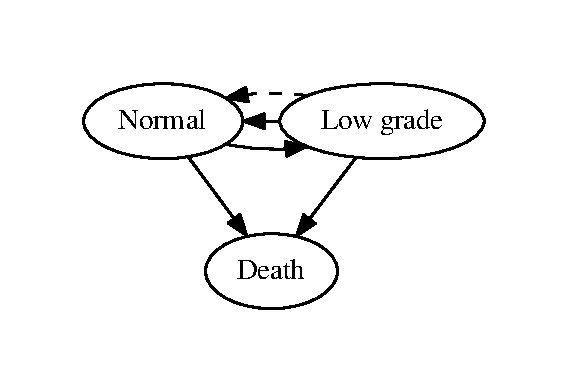
\includegraphics[width = 0.3\textwidth]{pic/M0}
	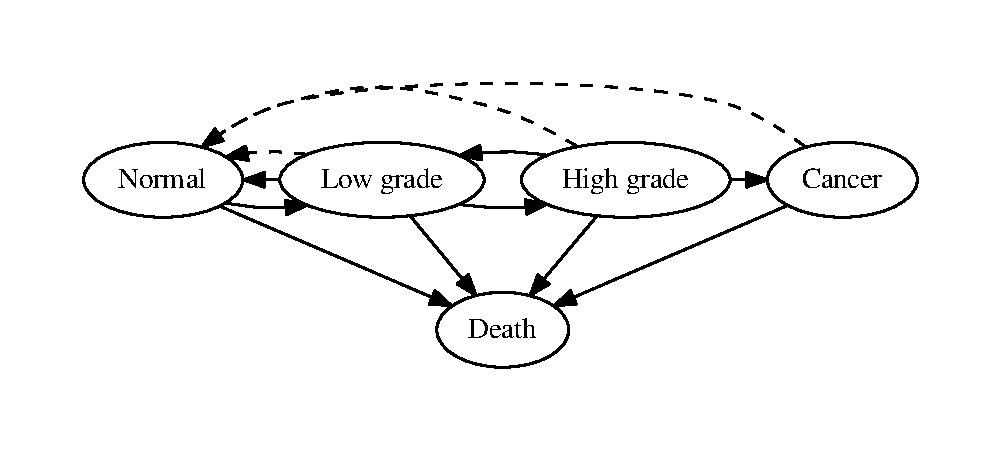
\includegraphics[width = 0.4\textwidth]{pic/M1}
	\caption{Transition structure of model $\mathcal{M}_0$ and $\mathcal{M}_1$. Solid lines denote the intensity transition while dashed lines denote that any state comes back to the normal state once treatment is completed.}
	\label{fig:HHMM}
\end{figure}

This hierarchical structure of the HIHMM allows for an arbitrary number of latent frailty states, provided relevant Markov models can be ascribed to the disease progression associated with each. The rest of this section describes this general HIHMM in detail.  

\subsection{Variables}
Suppose there are $N$ individuals in the screening population.  Let individual $n$ have $T_n$ screening visits at ages $a_1, \ldots, a_{T_n}$. We assume $Z$ categories are considered in the hierarchical frailty structure and introduce the following variables:
\begin{eqnarray}
\textrm{Frailty State (hidden):} & z_{n} \in \{1, \ldots, Z\} \nonumber \\
\textrm{Disease States (hidden):} & S_{nt} \in \{1, \ldots, M_{z_n}\} \nonumber \\
\textrm{Number of screening tests (observable):} & E_{ntk} \in \mathbb{N} \nonumber \\
\textrm{Screening test results (observable):} & G_{ntk} \in \mathbb{N}^{L_k} \nonumber 
\end{eqnarray}
The underlying disease state of individual $n$ is assumed to evolve according to a continuous-time, time-inhomogeneous Markov process assigned by its latent frailty class indicator $z_n$, where only screening results at specific time stamps with corresponding ages $a_1, \ldots a_{T_n}$ are observable. On the $t$th screening visit of individual $n$, $S_{nt}$ refers to the latent disease state and the visit includes $E_{ntk}$ tests of the $k$th test type and the corresponding results $G_{ntk}$, which is a $L_k$ dimensional vector and the value on $l$th dimension refers to the number of the $l$th grade results. 

\subsection{Model of Disease Progression}
As for the $z$th underlying Markovian disease process, it is parameterized by an $M_z \times M_z$ transition intensity matrix $Q_z$. For the simplicity of notation, we ignore the subscribe $z$ in the reminder of this section. The $ij$th element $q_{ij}$ of $Q$ satisfying $q_{ij} \geq 0$ for $i\neq j$ and $q_{ii} = -\sum_{i\neq j}q_{ij}$.    
The time spent in state $i$ is exponentially distributed with rate $-q_{ii}$.  Given that a transition occurs from state $i$,  the probability of transitioning to state $j$ is $\frac{q_{ij}}{q_i}$ where $q_i = \sum_{i\neq j}q_{ij}$.

As $Q$ is invariant for time $t$ the model is homogeneous, otherwise the model is inhomegeneous. We discuss homogeneous model and extend it to inhomegeneous model using piece-wise constant transition intensity matrix in Section~\ref{sec:homogeneous} and Section~\ref{sec:inhomogeneous} separately.

\subsubsection{Homogeneous Markov Model} \label{sec:homogeneous}
As for a homogeneous Markov process, we assume the initial state at $t_0$ is known, $p(S(t_1)) = 1$. We let $\bm t' = (t'_1, \ldots, t'_{T'})$ refer to underlying transition timestamps and let $\bm O = (O_1, \ldots, O_T)$ denote observations at time $\bm t = (t_1, \ldots, t_T)$. Then complete likelihood (CL) is given by 
\begin{eqnarray}
\mathrm{CL} & = & \prod_{i = 1}^{T'}(q_{S(t'_i),S(t'_{i+1})}/q_{S(t'_i)})q_{S(t'_i)}e^{-q_{S(t'_i)}\vartriangle_i} \prod_{j = 1}^Tp(O_j|S(t_j)) \nonumber\\
& = & \prod_{i = 1}^{M}\left(e^{-q_i\tau_i} \prod_{j\neq i} q_{ij}^{n_{ij}}\right)\prod_{j=1}^Tp(O_j|S(t_j))\,,
\label{CL}
\end{eqnarray}
where $\tilde{\vartriangle}_i = \tilde{t}_{i+1} - \tilde{t}_i$ and $n_{ij}$ denotes the number of times the state changes from state $i$ to state $j$ during the whole process and $\tau_i$ denotes the duration that the process stays in state $i$.

Since underlying transition timestamps $\bm t'$ are not observable, marginalized complete likelihood (MCL) is derived by marginalizing all $\bm t'$ as
\begin{equation*}
\mathrm{MCL} = \prod_{i = 1}^{T-1}P(\vartriangle_i)_{S(t_i), S(t_{i+1})}\prod_{j = 1}^T p(O_j|S(t_j)) \,,
\end{equation*}
where $\vartriangle_i = t_{i+1} - t_i$ and $P(\vartriangle_i) = e^{Q \vartriangle_i }$ is the transition probability matrix from time $t_i$ to time $t_{i+1}$.  

\subsubsection{Inhomogeneous Markov Model} \label{sec:inhomogeneous}

Inhomogeneous Markov process drops the time invariance assumption of $Q$, by assuming that $Q$ is a function of $t$. In this case, deriving the CL is intractable, because the time spent in state $i$ does not follow an exponential distribution. An alternative approach is to consider the MCL. The only difference of the expression of MCLs between homogeneity and inhomogeneity is the computation of the transition matrix $P([t_i, t_{i+1}])$ from time $t_i$ to time $t_{i+1}$ for $i = 1, \ldots, T - 1$. For the inhomogeneous model, $P([t_i, t_{i+1}]) = e^{\int _{t_i}^{t_{i+1}}Q(t)dt}$.

The transition intensity function $Q(t)$ can be modeled by any parametric model, but the computation of matrix exponential $e^{\int _{t_i}^{t_{i+1}}Q(t)dt}$ may be prohibitively expensive, even taking  advantage of numerical computational methods. To ease this computational burden, we propose a piecewise constant transition intensity matrix $Q$, where each element $q_{ij}$ is a piecewise constant function of time. Specifically, we partition time into $I$ disjoint intervals covering the range of observable time.  We then have a set of disjoint partitions $\mathcal{A} = \{ A_i\}_{i=1}^{I}$. Each transition intensity function $q_{ij}$ is then a piecewise constant function via the defined partition $\mathcal{A}$, denoted by $q_{ij}(t) = \sum_{k = 1}^{I}q_{ijk} \bm 1_{A_k}(t)$, where $\bm 1(\cdot)$ is a Kronecker delta function and $q_{ij\ell} \geq 0$. In the case, the inhomogeneous Markov process can be treated as a combination of several continuous-time homogeneous Markov processes. Specifically, the transition probability matrix $Q$ can be computed as a production of transition probability matrices with respect to their corresponding partitions.

\subsection{Hierarchical Model}

Due to the significance of population heterogeneity related to disease exposure risk, we propose the hierarchical model as follows. Let $\bm \psi = (\bm \psi_1, \ldots, \bm \psi_Z)$ denote all model parameters and $\bm \psi_z$ are parameters for model $z$. Then the hierarchical model is given by
\begin{eqnarray*}
	\bm O_n & \sim & \mathcal{M}_{z_n}(\bm \psi_{z_n}, \bm \theta_n) \\
	z_n & \sim & \mathrm{Cat}(\bm p)\,, 
\end{eqnarray*}
where $\bm \theta_n$ denote all covariates for individual $n$. An informative prior of the model indicator $z_n$ is proposed as a categorical distribution with hyper-parameters $\bm p$, which is used to provide expert knowledge of the model assignment. This prior contributes to reasonable model inference, especially when screening data are highly imbalanced in terms of latent class membership.    Figure~\ref{fig:HHMM} shows the case where $Z=2$ and index $z_n$ has a Bernoulli prior with a parameter $p$, i.e.\ $z_n \sim \mathrm{Ber}(p)$.


\section{Inference}
Due to the latent characteristics of both model indices and patient states, expectation maximization (EM) approach is considered. Moreover, considering the heterogeneity of our model, we marginalize the latent transition timestamps in our inference. 

Specifically, we decompose the joint posterior distribution by $p(z_n, \bm S_n| -) = p(z_n| - )p(\bm S_n| z_n, -)$ and use soft assignment for $p(z_n| -)$ and hard assignment for $p(\bm S_n| z_n, -)$, because the computation of $p(\bm S_n|z_n, -)$ is prohibitively expensive. For simplicity, we ignore covariates $\bm{\theta}_n$ in the reminder of this section. Then recursive procedures are given as follows.
\begin{itemize}
	\item Given previous estimates $\bm \psi^{(t-1)}$, compute the conditional posterior distribution of $z_n$:
	\begin{align}
	p(z_n|\bm O_n, \bm \psi^{(t-1)}) & \propto \mathrm{Cat}(z_n|\bm p)p(\bm O_n| z_n, \bm\psi^{(t-1)}_{z_n}) \nonumber \\
	& \sim \mathrm{Cat}(\tilde{\bm p}_n)\,,
	\label{Pos_I}
	\end{align}
	where $\tilde{p}_{nk} = \frac{p_k p(\bm O_n| z_n = k, \bm{\psi}^{(t-1)}_k)}{\sum_{z = 1}^{Z}p_z p(\bm O_n | z_n = z, \bm\psi^{(t-1)}_z)}$ for $k = 1, \ldots, Z$ and $p(\bm O_n | z, \bm \psi_{z})$ is accessible through the filter-forward backward-sample algorithm (FFBS), which is a sequential Monte Carlo approach first proposed in \cite{Kitagawa_1987}.
	\item Update the optimal state sequence $\bm S_n$ given corresponding observations $\bm O_n$ and model indicator $z$ using the Viterbi algorithm \citep{Forney_1973}: 
	\begin{align}
	\bm S^{(t)}_{nz} = \mathrm{Viterbi}(\bm O_n, \bm \psi_z)\,.
	\label{Pos_S}
	\end{align}
	\item Maximize the EMCLL with respect to $\bm \psi$ by
	\begin{align}
	\bm \psi^{(t)} & = \arg\max\limits_{\bm{\psi}}\sum_{n=1}^{N}E_{z_n, \bm S_n}(\ell(\bm \psi| \bm O_n, z_n, \bm S_n)| \bm O_n, \bm \psi^{(t-1)}) \nonumber \\ 
	% & = \arg\max\limits_{\bm{\psi}}\sum_{n = 1}^{N}\sum_{z = 1}^{Z}\sum_{\bm S_n} p(z_n = z| \bm O_n, \bm{\psi}^{(t-1)})  p(\bm S_n |z_n = z, \bm O_n, \bm{\psi}^{(t-1)})\ell(\bm \psi| \bm O_n, z, \bm S_n) \nonumber \\
	%	& = & \max\limits_{\bm{\psi}} \sum_{i = 1}^{I}\sum_{z = 0}^{1}p(z_i = z| \bm o_i, \bm \psi^{(t-1)})\bm 1_{\bm s_{iz}^{(t)}}(\bm s_i) \ell(\bm \psi| \bm o_i, z, \bm s_i) \nonumber \\
	% & =  \arg\max\limits_{\bm{\psi}} \sum_{n = 1}^{N}\sum_{z = 1}^{Z}p(z_n = z| \bm O_n, \bm \psi^{(t-1)}) \ell(\bm \psi| \bm O_n, z, \bm S^{(t)}_{nz}) \nonumber \\
	& =   \arg\max\limits_{\bm{\psi}} \sum_{n = 1}^{N}\sum_{z = 0}^{Z}p(z_n = z| \bm O_n, \bm \psi^{(t-1)})  \left(\log p_z + \log p(\bm S_n | z, \bm \psi) + \log p(\bm O_n| \bm S_n, \bm \psi) \right)\,.
	\label{M_step}
	\end{align}
\end{itemize}



\section{Experimental results}
The HIHMM is demonstrated on a true population-level cervical cancel screening test dataset from the Cancer Registry of Norway. Data used in the analyses will be available on request from the Cancer Registry of Norway, given legal basis according to the GDPR. We describe the full model and inference method as follows. 

\subsection{Data and Model Description}\label{sec:data}
This dataset contains 1.7 million patients' screening testing records. Moreover, each patient contains a censored observation at the last time stamp $t_{c}$. Censored observations are denoted by $O_{c}$ which indicates whether the woman is dead or alive at time $t_c$. Moreover, each patient has treatment indices to show when and how many treatments are accepted. Observation contains the number of screening tests of cytology, histology and hpv. Cytology and histology have four levels of grade while hpv has two levels.

We set $Z = 2$, the model processes are displayed in Figure~\ref{fig:HHMM}. For model $z$, the initial state  is model as  
\begin{eqnarray*}
	S_{z1}|a_{1} & \sim & \mathrm{Cat}(\bm \pi_z(\mathcal{A}, a_0)) \\
	\bm \pi_{zi} & \sim & \mathrm{Dir}(\bm \alpha_{zi})\,,
\end{eqnarray*}
where $a_1$ denotes the age at the first screening test and $\mathcal{A}$ is a disjoint partition of observable ages, $\bm \pi_z(\mathcal{A}, a) = \bm \pi_{zi}$ if and only if $a \in \mathcal{A}_{i}$, and $\bm{\alpha}_{z\ell} \in \mathbb{R}^{+M_z}$.

The observations $\bm O$ have two levels: the number of screening tests $\bm E$ and the results of screening tests $\bm G$. Remove the subscripts $n$ and $t$. Given state $s$, observations are modeled as  
\begin{eqnarray*}
	E_k & \sim & \mathrm{Poisson}(\eta_{sk})\,, \nonumber \\
	{\bm G}_k|E_k & \sim & \mathrm{Multinomial}(E_k, \tilde{\bm\pi}_{sk})\,, \nonumber \\
	\tilde{\bm\pi}_{sk} & \sim & \mathrm{Dir}(\tilde{\bm\alpha}_{sk}) \,,
\end{eqnarray*}
where 
$\tilde{\bm \alpha}_{sk} \in \mathbb{R}^{+L_k}$ are hyper-parameters for observation model.

And the censored observation (dead or alive) is modeled by
\begin{eqnarray*}
	p(O_{c}|S_T) = \begin{cases}
		P(t_T, t_{c})_{S_T, \text{death}} & \text{ if } O_{c} = \mathrm{death}\\
		1-P(t_T, t_{c})_{S_T, \text{death}} &   \text{ if }  O_{c} \neq \mathrm{death}\,.
	\end{cases}
\end{eqnarray*}

Treatment modeling and inference are discussed in Appendix~\ref{sec:treatment}. Age partition selection is discussed in Appendix~\ref{sec:age}. Finally we choose the age partition as $\mathcal{A}$ as $[0, 23)$, $[23,30)$, $[30,60)$ and $[60, \infty)$. As for model training, optimization is discussed in Appendix~\ref{sec:pars_transformation}
 and hyper-parameters is discussed in Appendix~\ref{sec:opt_set}.

\subsection{Model Comparison}
We randomly select 80000 patients' records for training and select other 20000 patients' records for testing. The goal is to predict the last visiting status and the status is defined based on the observations at the last visit. Specifically, if a patient has at least one result whose level is greater than 1, then the status is defined as high risk denoted as $1$. Otherwise, the status is defined as low risk denoted as $0$. Thus, the problem is defined as a binary classification problem. 

The prediction procedure is defined as follow. After model training, let model parameter estimates be $\hat{\bm \psi}$. Given new patient historical records $\bm O^*$, compute the predictive distribution of model index $p(z^*|\bm O^*, \hat{\bm \psi})$. Next, Given model index $z$, compute predictive distribution of state at the last second visiting 
$p(S^*_{T-1}|z, \bm O^*, \hat{\bm \psi})$ derived from FFBS. Then predictive distribution of state of the last visiting is 
$p(S^*_{T}|\bm O^*, \hat{\bm \psi}) \sum_{z} p(z^* = z|\bm O^*, \hat{\bm \psi}) p(S^*_{T}|z, \bm O^*, \hat{\bm \psi})$ and predictive distribution of screening test results are $p(\bm G^*_{T}| \bm O^*, \bm E^*_T, \hat{\bm \psi}) = \sum_s p(S^*_{T} = s|\bm O^*, \hat{\bm \psi}) p(\bm G^*_{T}| S_{T}^* = s, \bm E_{T}^*, \hat{\bm \psi})$. Finally, the predictive distribution of the last status is $G^* \sim \mathrm{Ber}\left( p^* \right)$, where $p^* = p\left(\sum_{i = 0}^{1}\sum_{j = 2}^3 \bm G_{T}^*[i,j] \geq = 1 |  \bm O^*, \bm E^*_T, \hat{\bm \psi}\right)$. and it is estimated by $\hat{G^*} = \begin{cases}
1 & p^* \geq 0.5 \\
0 & \mathrm{otherwise} \\
\end{cases}$.

As for state of the art recurrent neural network models, each patient's record is modeled as one time-series and the features at each visit includes patient's age, patient's screening result and patient's treatment indicator. Specifically, screening result of patient $n$ at $t$th visiting is $\vec{\bm G_{n,t}}$. And treatment indicator is a binary number, it is equal to 1 if and only if the patient has accepted treatment. LSTM \citep{Cho_2014}, stacked LSTM \citep{Dyer_2015} and GRU \citep{Chung_2014} are implemented for model comparison. As for stacked LSTM, two LSTMs are stacked. We summarize prediction results in Table~\ref{Model_Comparison}. It shows our model outperforms state of the art methods in term of Area Under The Curve(AUC). And HIHMM with prior setting $p = 0.2$ obtains the best prediction performance.

\begin{table}[ht!]
	\centering
	\caption{Model prediction for the status of the last visit in terms of Accuracy (ACC), Area Under The Curve(AUC), True Positive (TP), False Positive (FP), True Negative (TN) and False Negative (FN).}
	\begin{tabular}{|c|c|c|c|c|c|c|c|}
		\hline
		Method & Prior & ACC & AUC & TP & FP & TN & FN \\
		\hline
		LSTM &  & 0.9920 & 0.85 & 43 & 147 & 19779 & 13 \\
		\hline
		stacked LSTM &  & 0.9914 & 0.86 & 39 & 151 & 19788 & 22 \\
		\hline
		GRU &  & 0.9922 & 0.85 & 59 & 131 & 19786 & 24 \\
		\hline
		HIHMM & 0.2 & 0.9916 & 0.9098 & 73 & 117 & 19759 & 51 \\
		\hline
		HIHMM & 0.3 & 0.9916 & 0.9095 & 56 & 134 & 19776 & 34 \\
		\hline
		HIHMM & 0.4 & 0.9918 & 0.8997 & 53 & 137 & 19782 & 28 \\
		\hline
		HIHMM & 0.5 & 0.9917 & 0.8995 & 53 & 137 & 19781 & 29 \\
		\hline
	\end{tabular}
	\label{Model_Comparison}
\end{table}


\subsection{Model Validation}
We set model index prior $p = 0.2$ based on model comparison results and expert opinion. And we present two types of results on population-level data. First we present the MLEs for all model parameters along with bootstrapped standard deviations. Second we perform model validation using Kaplan-Meier estimators as suggested in \cite{titman_general_2008}.

\subsubsection{Parameter Estimation}
We randomly divide all data into clusters such that each cluster has 100 individual observation sequences. Using a bootstrap technique, we randomly select $2400$ clusters with replacements for model inference. We independently repeat the same inference on different selections 5 times. The mean and standard deviation of all parameter estimates are discussed in Appendix~\ref{sec:pars}.

\subsubsection{Model Validation}
For model validation we randomly select $2400$ clusters of data in which each cluster has 100 individual sequences of observations. We implement both the HIHMM and the CTIHMM for the same dataset. We follow the method proposed in \cite{titman_general_2008} that utilizes Kaplan-Meier estimators to validate continuous-time HMMs. Kaplan-Meier estimators are defined according to the definition of a failure, or time-to-event. In multi-state models different failures can be defined depending on which features of the model and data are of interest. Here we define failure as the first observation of a high-risk or cancer test result directly following an initial normal or low-grade test result.  Accurately predicting this time-to-event is of practical importance because clinical intervention is only possible in the high-grade state.  Treating patients at this stage is critical to preventing precancerous lesions from progressing to cervical cancer. 

The empirical Kaplan-Meier estimator is defined as 
\begin{eqnarray*}
	\hat{S}(t) = \prod_{i: t_i\leq t}\left(1 - \frac{d_i}{n_i}\right)\,,
\end{eqnarray*}
where $t_i$ a time when at least one failure is observed, $d_i$ is the number of failures that occurred at time $t_i$, and $n_i$ is the number of individuals known to have survive up to time $t_i$. We randomly choose $24000$ records to generate an empirical Kaplan-Meier estimator according to our definition of a failure. Furthermore, we generate Kaplan-Meier estimates by simulating $100$ sequences from both the CTIHMM and HIHMM and repeat this $100$ times. Figure~\ref{KM_PF} shows the empirical Kaplan-Meier curve in black, simulated Kaplan-Meier curves from the CTIHMM in blue, and simulated Kaplan-Meier curves from the HIHMM. As for the simulated Kaplan-Meier curves, solid lines denote the median curve and dashed lines denote the 95\% credible intervals based on the 100 replications. The results show that the empirical Kaplan-Meier curve is always near the median and within the 95\% credible intervals generated by the HIHMM. This is not the case with the CTIHMM. In this sense the HIHMM outperforms the CTIHMM in an important clinical metric.

On the other hand, the HIHMM has a relatively high Kaplan-Meier estimate at time $0$ because the informative prior $p = 0.2$ is relatively small. This has the effect of driving simulated patients to more likely be in the low-risk model $\mathcal{M_0}$ at the initial time. Moreover, these patients are more likely to stay at the normal state for longer. However, the trend of the median curve from the HIHMM more closely tracks that of the empirical Kaplan-Meier curve, compared with the trend of the median curve from the CTIHMM. This suggests that the HIHMM models disease progression better than the CTIHMM. The Kaplan-Meier curves simulated from the CTIHMM are always underestimated.
\begin{figure}
	\centering
    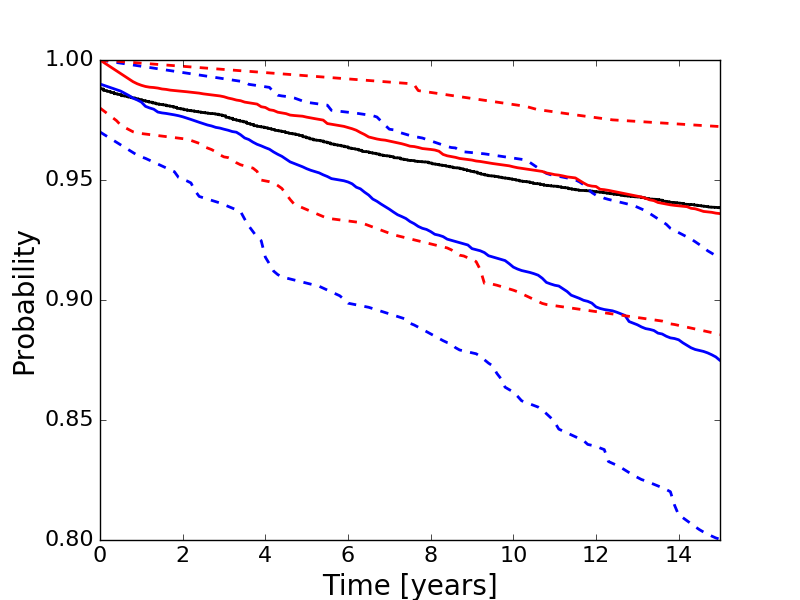
\includegraphics[width = 0.45\textwidth]{pic/hmm/KM_curve_shared_version1}
    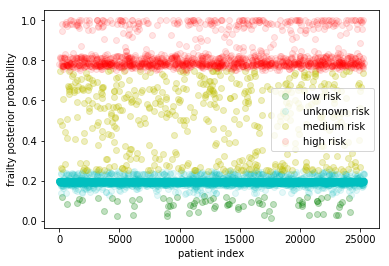
\includegraphics[width = 0.45\textwidth]{pic/hierarchical-hmm-posterior-frailty-probs.png}
	\caption{Left panel: Empirical Kaplan-Meier curve (black) and simulated Kaplan-Meier curves, which are summarized using the 95\% credible interval (dashed lines) and the median (solid lines), from the CTIHMM (blue) and HIHMM (red). Right panel: Posterior probabilities of belonging to the frailty class for each individual from a test set. Risk stratification is possible by thresholding the probabilities. Threshold probabilities in this example are $(0, 0.125,0.25, 0.75,1)$. Color indicates falling between two probability thresholds.}
	\label{KM_PF}
\end{figure}

\section{Discussion and Conclusion}
One of the possible applications of the HIHMM in the context of population-based screening programs is risk stratification of the population.  The latent random variable $z_n$ is an indicator of belonging to a frail class in the population.  Given the learned model parameters $\bm \psi$  it is possible to compute the posterior probability of belonging to the frailty class for individual women.  In other words, given an observed sequence of test results ${\bm O}_n$ and model parameters  $\bm \psi$,  the posterior predictive distribution $p(z_n | \psi, {\bm O}_n)$ is of interest.  This parameter gives a measure of the likelihood of an individual to be at risk of developing cervical cancer conditioned on their observed test results. Such information could be used to more efficiently screen a population by avoiding the over screening of women at low-risk and the under screening of women at high-risk.  


Examples of these posterior probabilities are shown in Fig \ref{KM_PF}. For illustration purposes, we have chosen risk thresholds of $\{0.125,0.25, 0.75\}$ with the following interpretation.
\begin{align*}
0 \leq p(z_n | \bm \psi, {\bm O}_n) < 0.125 &\implies \text{ low-risk  } \\
0.125 \leq p(z_n | \bm \psi, {\bm O}_n)  < 0.25 &\implies \text{ unknown risk  }\\
0.25 \leq p(z_n | \bm \psi, {\bm O}_n)  < 0.75      &\implies \text{ medium-risk }\\
0.75 <  p(z_n | \bm \psi, {\bm O}_n) \leq 1 &\implies \text{ high-risk } 
\end{align*}

Two main clusters are apparent in the data corresponding to unknown risk and high risk. The unknown risk cluster is those patients close to the prior probability of $20\%$.  These patients lack sufficient observations to make an informed decision about their risk profile.  This suggests these patients should be followed up with the standard screening protocol.  The high risk cluster is those patients which are more likely to be in a high-grade state.  This suggests these patients may require immediate follow up.  The two smaller clusters of low risk and medium risk are comprised of patients that may require decreased or increase screening frequencies, respectively, relative to the standard screening protocol. 


In summary, this paper has made the following contributions:
\begin{itemize}
	\item We make CTIHMM inference for population-level datasets possible by using piece-wise constant intensity functions and deriving a scalable inference algorithm.
	\item We put a hierarchical structure over the CTIHMM to explain population heterogeneity in terms of frailty, resulting in our HIHMM.
	\item We utilize prior distributions in the model to achieve more accurate estimates when data is scarce.    
	\item We perform full model inference and prediction on subset of cancer screening dataset and show that our model outperforms other state of the art recurrent neural network models on the prediction task.
	\item We perform full model inference on a population-level cancer screening dataset and show that population heterogeneity improves model performance in terms of Kaplan-Meier estimators. 
	\item We illustrate how the model may be used to better inform public health professionals by providing a risk stratification mechanism. 
\end{itemize}


\newpage
\bibliographystyle{plainnat}
\bibliography{ref}

\newpage
\section{Supplemental Materials for Reproducibility}
\subsection{Treatment Modeling}\label{sec:treatment}
Because of treatments, the inference has three modifications for FFBS, Viterbi and EMCLL. Without loss of generality we suppose one woman has $m$ treatments indexed by $\{r_1, \ldots, r_m\}$. Then the observation sequence $\bm O$ is partitioned as 
$$\{\bm O_1, \ldots, \bm O_{r_1}\}, \ldots, \{\bm O_{r_m}, \ldots \bm O_T, \bm O_{c} \}.$$

Throughout the FFBS, the marginal likelihood is decomposed as
\begin{align}
p(\bm O |z, \bm \psi) & = p(\bm O_1, \ldots, \bm O_{r_1}| z, \bm \psi) \prod_{j = 1}^{m-1}p(\bm O_{r_j+1}, \ldots, \bm O_{r_{j+1}}| S_{r_j} = 0, z, \bm \psi) \nonumber \\
& \qquad p(\bm O_{r_m+1}, \ldots \bm O_T, \bm O_{c}| S_{r_m} = 0, z, \bm \psi). 
\label{FFBS}
\end{align}
Each component of (\ref{FFBS}) is tractable using FFBS \cite{Kitagawa_1987}.

A similar decomposition is implemented in the Viterbi algorithm to find the most likely sequence of hidden states.
\begin{align}
(S_1, \ldots, S_{r_1}) & = \mathrm{Viterbi}(\bm O_1, \ldots, \bm O_{r_1}, \bm \psi)\,, \nonumber \\
(S_{r_j+1}, \ldots, S_{r_{j+1}}) & = \mathrm{Viterbi}(\bm O_{r_j+1}, \ldots, \bm O_{r_{j+1}}, \bm \psi| S_{r_j} = 0)  \nonumber \\
& \qquad j = 1, \ldots, m-1\,,  \nonumber \\
(S_{r_m}, \ldots, S_{T}) & = \mathrm{Viterbi}(\bm O_{r_m+1}, \ldots, \bm O_{T}, \bm O_{c}, \bm \psi | S_{r_m} = 0) \,.
%(S_{r_m}, \ldots, S_{T}) & = \mathrm{Viterbi}(\bm O_{r_m+1}, \ldots, \bm O_{T}, \bm O_{c}, \bm \psi \nonumber \\& \qquad| S_{r_m} = 0) \,.
\end{align}

According to (\ref{M_step}), to compute EMCLL we only need to compute $p(\bm S| z, \bm{\psi})$. Using a similar decomposition we arrive at
\begin{eqnarray*}
	p(\bm S|z, \bm\psi) =  p(S_1|z, \bm \psi)\prod_{i \in \{r_j\}} p(S_{i+1}| S_i=0) \prod_{i \notin \{r_j\}, i \neq 1} p(S_{i+1}| S_i).
\end{eqnarray*}


\subsection{Age Segmentation} \label{sec:age}
Since HPV status is one of most import indicator for cervical censor, we segment the age interval based on the empirical density of ages at which patients find positive HPV. The empirical density is estimated based on 100000 patients randomly sampled from the pool using gaussian kernel estimation. Then we fit the density of ages using discontinuous piece-wise linear function with different number of intervals. 

Fitting information is summarized in Table~\ref{age_segmentation}. We plot optimal sum of square errors under different $N$ in Figure~\ref{age_segmentation_plot}. From the figure, it visually shows that $N=4$ is the optimal number of segmentation based on elbow criteria. Then combining the expert's opinion, we set the corresponding cutting points as $[23,30,60]$. 

\begin{table}[ht!]
	\centering
	\caption{Discontinuous piece-wise linear fitting under different number of intervals $N$. Optimal sum of square errors (SSE) and cutting points (CPs) are given.}
	\label{age_segmentation}
	\begin{tabular}{|c|c|c|}
		\hline
		$N$ & SSE & CPs\\
		\hline
		2 & 3.88e-3 & 24.8 \\
		\hline
		3 & 1.78e-3 & 24.7, 54.7 \\
		\hline
		4 & 1.23e-3 & 25.2, 35.6, 60.6  \\
		\hline
		5 & 0.93e-3 & 24.5, 26.2, 30.7, 67.2 \\
		\hline
		6 & 0.78e-3 & 24.1, 25.2, 32.8, 56.9, 64.4 \\
		\hline
	\end{tabular}
\end{table}

\begin{figure}[ht!]
	\centering
	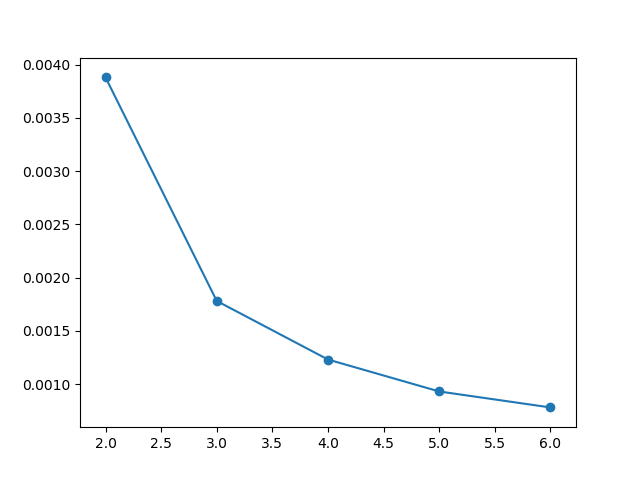
\includegraphics[scale=0.5]{pic/hmm/sse_vs_n}
	\caption{Sum of square errors under different number of segmentation $N$.}
	\label{age_segmentation_plot}
\end{figure}


\subsection{Parameter Transformation in Limited-Memory BFGS Optimization} \label{sec:pars_transformation}
In the HIHMM, model parameters $\bm \psi$ are summarized as follows:
\begin{itemize}
	\item Emission parameters $\tilde{\bm \alpha}_{sk} > 0$ and $\eta_{sk} > 0$ for $s = 1, \ldots M$ and $k = 1,\ldots, K$.
	\item Initial state parameters $\bm \alpha_{zi} > 0$ for $z = 1,\ldots, Z$ and $i = 1, \ldots, |\mathcal{A}|$.
	\item Unconstrained transition intensity parameters $\bm \lambda_{zi} > 0$ for $z = 1,\ldots z$ and $i = 1, \ldots, |\mathcal{A}|$.
\end{itemize}

In the M-step, all model parameters need to be optimized. To take advantage of the L-BFGS approach, we need to transform the constrained optimization problem to an unconstrained optimization problem. To do this we transform all parameters on the log scale, which means we let $\tilde{\bm \alpha}^* = \log {\tilde{\bm \alpha}}$, $\bm\eta^* = \log \bm \eta$, $\bm \alpha^* = \log \bm \alpha$ and $\bm \lambda^* = \log \bm \lambda$. Then we let $\bm \psi^* = (\tilde{\bm \alpha}^*, \bm \eta^*, \bm \alpha^*, \bm \lambda^*)$. Finally we maximize the EMCLL with respect to $\bm \psi^*$ rather than $\bm \psi$. After the optimization, the optimized $\hat{\bm \psi}$ are accessed by $\hat{\bm \psi} = \exp(\hat{\bm \psi}^*)$.

\subsection{Optimization Settings} \label{sec:opt_set}
In the proposed learning approach, we set the number of EM iterations at $N_{EM} = 100$, and in the L-BFGS approach we set the number of optimization iterations as $N_{L-BFGS} = 8$. The automatic differentiation is implemented using the autograd package \cite{Maclaurin_2016} in Python.


\subsection{Parameter Estimation} \label{sec:pars}
Table~\ref{Table_1} shows more than $75\%$ of women have a posterior probability of belonging to the high-risk model $\mathcal{M}_1$ that is less than the prior probability $p = 0.2$. This suggests that more than $75\%$ are likely to be in the low-risk disease exposure category according to their screening test results. Moreover, it also justifies the expert knowledge that around $20\%$  belong to the high-risk disease exposure category. Whereas, the $90\%$ credible interval of the posterior hyper-parameter $\tilde{p}$ is $(0.1825, 0.2358)$, which is still close to the prior hyper-parameter $p = 0.2$. 
%This implies that the observations do not affect the posterior of model indexes significantly and so the prior is pretty important in the HIHMM.
This implies that the observations do not affect the posterior of the model indexes significantly and choosing a reasonable prior is important.  This is likely an artifact of the dataset, which is highly skewed towards normal test results.  More balanced datasets may exhibit less sensitivity to prior specification. 

\begin{table}[ht!]
	\centering
	\caption{Maximum likelihood estimates of quantiles of the posterior probability for Model 1.}
	\label{Table_1}
	\resizebox{\columnwidth}{!}{
		\begin{tabular}{|c|c|c|c|c|c|}
			\hline
			quantiles & 0.05 & 0.25 & 0.5 & 0.75 & 0.95 \\
			\hline 
			$\tilde{p}$ & 0.1825(0.0004) & 0.1936(0.0001) & 0.1966(0.0002) & 0.1988(0.0001) & 0.2358(0.0049) \\
			\hline
		\end{tabular}
	}
\end{table}


In Table~\ref{Table_2}, the estimates of diagnostic test results match the definition of states. The more advanced a patient's disease state, the more likely she is to get an abnormal screening result. The small standard deviations suggest that our data is sufficient to get precise estimates of the emission parameters. 

\begin{table}[ht!]
	\centering
	\caption{Maximum likelihood estimates of diagnostic test result probabilities conditioned on hidden state.}
	\label{Table_2}
	\resizebox{\columnwidth}{!}{
		\begin{tabular}{|c|c|c|c|c|}
			\hline
			\multicolumn{5}{|c|}{cytology}\\
			\hline
			state & 0 & 1 & 2 & 3 \\
			\hline
			normal & 1.0000(0.0000) & 0.0000(0.0000) & 0.0000(0.0000) & 0.0000(0.0000)\\
			low grade & 0.0331(0.0011) & 0.8021(0.0020) & 0.1631(0.0019) & 0.0016(0.0001)\\
			high grade & 0.0614(0.0068) & 0.0054(0.0010) & 0.9198(0.0059) & 0.0133(0.0012) \\
			cancer & 0.0619(0.0125) & 0.0567(0.0084) & 0.6254(0.0158) & 0.2560(0.0097) \\
			\hline
		\end{tabular}
	}
	\bigskip
	
	\resizebox{\columnwidth}{!}{
		\begin{tabular}{|c|c|c|c|c|}
			\hline
			\multicolumn{5}{|c|}{histology} \\
			\hline		
			state & 0 & 1 & 2 & 3 \\
			\hline
			normal & 0.9879(0.0004) & 0.0108(0.0004) & 0.0007(0.0001) & 0.0006(0.0001) \\
			low grade & 0.2621(0.0023) & 0.1561(0.0006) & 0.5810(0.0030) & 00009(0.0002) \\
			high grade & 0.0345(0.0018) & 0.0068(0.0015) & 0.9573(0.0026) & 0.0014(0.0001) \\
			cancer & 0.0263(0.0062) & 0.0133(0.0015) & 0.0796(0.0014) & 0.8808(0.0066) \\
			\hline
		\end{tabular}
	}
	
	\bigskip
	\resizebox{0.5 \columnwidth}{!}{
		\begin{tabular}{|c|c|c|}
			\hline
			\multicolumn{3}{|c|}{HPV} \\
			\hline
			state & - & +  \\
			\hline
			normal & 0.9966(0.0010) & 0.0034(0.0010) \\
			low grade & 0.3720(0.0048) & 0.6280(0.0048) \\
			high grade & 0.0357(0.0054) & 0.9643(0.0054) \\
			cancer & 0.0194(0.0019) & 0.9806(0.0019) \\
			\hline
		\end{tabular}
	}
	
\end{table}

Results from Table~\ref{Table_3} show the number of screening tests for women in different states. Due to the fact that the expectation of a Poisson distribution is exactly the Poisson intensity parameter, the Poisson intensities shows that individuals at normal state are more likely to be assigned to a cytology screening test. Individuals in abnormal disease states (low-grade, high-grade and cancer) are more likely to be given histology and HPV tests. This result matches what is expected in clinical practice in that women will be assigned more precise screening tests as they present more severe symptoms.

\begin{table}[ht!]
	\centering
	\caption{Maximum likelihood estimates of Poisson intensities for the number of tests conditioned on true state.}
	\label{Table_3}
	\resizebox{\columnwidth}{!}{
		\begin{tabular}{|c|c|c|c|}
			\hline
			state & cytology & histology & HPV \\
			\hline
			normal & 0.9880(0.0002) & 0.0140(0.0001) & 0.0053(0.0001) \\
			low grade & 0.7912(0.0008) & 0.1856(0.0018) & 0.1003(0.0016) \\
			high grade & 0.4595(0.0024) & 0.6493(0.0018) & 0.0290(0.0017) \\
			cancer & 0.5091(0.0191) & 0.8627(0.0322) & 0.0278(0.0023) \\
			\hline
		\end{tabular}
	}
\end{table}

Table~\ref{Table_4} shows the initial information of the population categorized by the specified age partition for model $\mathcal{M}_0$ and model $\mathcal{M}_1$. From a model specification perspective, women in the low-risk model, $\mathcal{M}_0$, are assumed to be more likely to stay at a normal state than women in the high-risk model $\mathcal{M}_1$, regardless of their ages. On the other hand, in the high-risk model, $\mathcal{M}_1$, women in the age interval $(23, 30)$ are mostly like to belong to a high risk state at the initial screening test. 

\begin{table}[ht!]
	\centering
	\caption{Maximum likelihood estimates of the probability of being a particular state at the time of the first screening.}
	\label{Table_4}
	\resizebox{\columnwidth}{!}{
		\begin{tabular}{|c|c|c|c|c|}
			\hline
			age range & 16-23 & 23-30 & 30-60 & 60- \\
			\hline
			\multicolumn{5}{|c|}{Model 0} \\
			\hline 
			normal & 0.9315(0.0010) & 0.9415(0.0017) & 0.9614(0.0007) & 0.9643(0.0009) \\
			low grade & 0.0685(0.0010) & 0.0585(0.0017) & 0.0386(0.0007) & 0.0357(0.0009) \\
			\hline
			\multicolumn{5}{|c|}{Model 1} \\
			\hline 
			normal & 0.9187(0.0015) & 0.9040(0.0011) & 0.9287(0.0006) & 0.9308(0.0020) \\
			low grade & 0.0761(0.0013) & 0.0677(0.0022) & 0.0438(0.0011) & 0.0354(0.0016) \\
			high grade & 0.0041(0.0003) & 0.0271(0.015) & 0.0262(0.0007) & 0.0263(0.0018) \\
			cancer & 0.0011(0.0001) & 0.0013(0.0002) & 0.0013(0.0002) & 0.0075(0.0006) \\
			\hline
		\end{tabular}
	}
\end{table}

Table~\ref{Table_5} displays the estimates of transition intensities in the two models. It shows patients are more likely to transition from the low grade state to the normal state, whether or not they are in model $\mathcal{M}_0$ or model $\mathcal{M}_1$. On the other hand, $\lambda_{34}$ has significantly higher standard deviations than other intensity parameters because of the scarcity of data for individuals with cancer who died during the period in which the data was collected. 

\begin{table}[ht!]
	\centering
	\caption{Maximum likelihood estimates for age dependent transition intensities.}
	\label{Table_5}
	\resizebox{\columnwidth}{!}{
		\begin{tabular}{|c|c|c|c|c|}
			\hline
			age range & 16-23 & 23-30 & 30-60 & 60- \\
			\hline
			\multicolumn{5}{|c|}{Model 0} \\
			\hline 
			$\lambda_{01}$ & 0.1718(0.0061) & 0.0809(0.0017) & 0.0546(0.0006) & 0.0439(0.0015) \\
			$\lambda_{02}$ & 0.0005(0.0000) & 0.0018(0.0000) & 0.0019(0.0000) & 0.0147(0.0001) \\
			$\lambda_{10}$ & 1.7064(0.0327) & 1.2637(0.0292) & 0.4893(0.0118) & 2.2169(0.0641) \\
			$\lambda_{12}$ & 0.0024(0.0002) & 0.0021(0.0001) & 0.0011(0.0001) & 0.0122(0.0013) \\
			\hline
			\multicolumn{5}{|c|}{Model 1} \\
			\hline 
			$\lambda_{01}$ & 0.1938(0.0065) & 0.1191(0.0032) & 0.0730(0.0011) & 0.0536(0.0020) \\
			$\lambda_{04}$ & 0.0014(0.0001) & 0.0015(0.0001) & 0.0015(0.0001) & 0.0121(0.0002) \\
			$\lambda_{10}$ & 1.6854(0.0295) & 1.3541(0.0358) & 1.6331(0.0131) & 2.3063(0.1288) \\
			$\lambda_{12}$ & 0.0815(0.0086) & 0.2276(0.0015) & 0.1867(0.0030) & 0.2395(0.0090) \\
			$\lambda_{14}$ & 0.0058(0.0003) & 0.0048(0.0002) & 0.0032(0.0003) & 0.0150(0.0006) \\
			$\lambda_{21}$ & 0.3585(0.0593) & 0.0780(0.0067) & 0.0663(0.0052) & 0.2245(0.0288) \\
			$\lambda_{23}$ & 0.0720(0.0095) & 0.0307(0.0017) & 0.1012(0.0060) & 0.5166(0.0366) \\
			$\lambda_{24}$ & 0.0150(0.0004) & 0.0069(0.0007) & 0.0034(0.0003) & 0.0166(0.0006) \\
			$\lambda_{34}$ & 1.0366(0.0611) & 2.5642(0.5100) & 2.6911(0.1251) & 1.6805(0.3432) \\
			\hline
		\end{tabular}
	}
\end{table}


\subsection{Simulations of Kaplan-Meier Curves}
To simulate one Kaplan-Meier curve from a HIHMM, we propose the following procedures:
\begin{itemize}
	\item[1] First, reduce all individuals' ages at their first screening test to a set $A_1$, and categorize individuals' time intervals between two consecutive screening tests into four sets denoted as $\tilde{I}_i$ for $i = 0,\ldots 3$. Any time interval $(a, b)$ is categorized into $\tilde{I}_i$, if and only if the largest value of both cytology and histology screening test results at time $a$ is $i$. Then for each set $\tilde{I}_i$, we map elements of $\tilde{I}_t$ to their corresponding lengths and name the new set as $I_i$  Also, we reduce all posterior probabilities of model indexes into a set $\tilde{P}$.
	\item[2] Second, we sample an initial age $a_1$ from $A_1$ and sample a posterior probability of model index $\tilde{p}$ from $\tilde{P}$.
	\item[3] Then sample model index $z$ by $z \sim \mathrm{Ber}(\tilde{p})$ and sample an initial state $S_1 \sim \mathrm{Cat}(\hat{\bm \pi}_z(\mathcal{A}, a_1))$, where $\hat{\bm \pi}_{zi} = \hat{E}(\bm \pi_{zi}) = \frac{\hat{\bm \alpha}_{zi}}{\sum \hat{\bm \alpha}_{zi}}$.
	\item[4] Based on current state $S_{t-1}$ and current age $a_{t-1}$ , sample the screening time interval $\Delta_{t-1}$ from $I_{S_{t-1}}$. Then compute transition matrix $P([a_{t-1}, a_{t}]| \mathcal{A}, \hat{\bm \lambda}_z)$ from age $a_{t-1}$ to $a_{t} = a_{t-1} + \Delta {t-1}$. Then sample $S_{t}$ by $S_{t} \sim \mathrm{Cat}(P[a_{t-1}, a_{t}]_{S_{t-1},:}) $.
	\item[5] Continue previous sampling processes until the state $S_T$ fails according to the failure definition of Kaplan-Meier estimator. Then compute the failure time by $F = \sum_{t = 1}^{T}\Delta_t$.
	\item[6] Repeat [2] to [5] $M$ times. We obtain $M$ failure times and then order them as a sequence $\{F_m\}$. 
	\item[7] Based on the simulated failure times $\{F_m\}$, the simulated curve is $S(t) = 1 - \frac{1}{M}\sum_{m: t \geq F_m}1$.
\end{itemize}
Multiple Kaplan-Meier curves are simulated by independently repeating the above procedures.

\end{document}
